\documentclass[../thesis.tex]{subfiles}

\begin{document}

    \chapter{Analysis}
    \label{ch:analysis}


      \section{Isotherm computation}
      \label{sec:isotherm-computation}

        In the following, evaluation of the recorded raw data is presented for volumetric (\cref{subsec:volumetric-computation}) and for the optical measurements (\cref{subsec:optical-computation}).


        \subsection{Volumetric isotherm}
        \label{subsec:volumetric-computation}


          To compute the isotherms from the recorded data the experiment needs to the conducted not only with a membrane inside of the cell, but also with an empty cell. From here on, the following indices shall be used:
          \begin{align*}
              \begin{split}
                  &1 \longrightarrow \textrm{no membrane} \\
                  &2 \longrightarrow \textrm{membrane}.
                  \label{eq:index_assignments}
              \end{split}
          \end{align*}
          Furthermore, the variables $P_i$, $\dot{P}_i$, $V_i$, $T_i$, $n_i$ and $\dot{n}_i$, $i\in \{1,2\}$, refer to the values measured inside of the cell, in explanation the red marked part of the system in \cref{fig:setup-bypass}. The raw isotherms of the two experiments are shown in \cref{fig:raw-isotherms}. The plateaus of the yellow curve with membrane inside the cell of the plot versus time  correspond to the dips of the time derivative of the pressure of the versus pressure plot. This can be explained by the hexane condensing inside the membrane's pores at a given pressure due to which the continuing matter flow into the cell does not yield an increase of pressure.
          \medskip

          \subfile{tikz/graphs/295b_membrane_vs_nomembrane/295b_membrane_vs_nomembrane.tex}

          Regarding the system with and empty cell, it is clear that the ideal gas law can be used to compute the flow rate of hexane (compare \cref{sec:ideal-gas-law}). By solving for the amount of matter
          \begin{equation*}
              n_1 = \frac{P_1V_1}{RT_1},
          \end{equation*}
          taking into account that the temperature of the cell is regulated at $T_1$ and the volume $V_1$ is constant, the flow of matter becomes
          \begin{equation*}
              \dot{n}_1 = \frac{V_1}{RT_1}\cdot \dot{P}_1.
              \label{eq:n1}
          \end{equation*}
          Furthermore, the flow of matter for the system with a membrane inside the cell can be interpreted as the sum of the flow into the membrane $\dot{n}_2^\mathrm{mem}$ and the flow into the system volume excluding the membrane $\dot{n}_2^\mathrm{cell}$. This can be rewritten yielding
          \begin{equation*}
              \dot{n}_2^\mathrm{mem} = \dot{n}_2 - \dot{n}_2^\mathrm{cell},
          \end{equation*}
          where $\dot{n}^\mathrm{cell}_2$ obeys ideal gas law. Using the fact that the flow through the \textsc{Pfeiffer} valve only depends on the pressure difference $\Delta P_i = P_i^\mathrm{tank} - P_i^\mathrm{cell}$, assuming that $P_1^\mathrm{tank} = P_2^\mathrm{tank}$ leads to
          \begin{align}
              \begin{split}
                  \dot{n}_2^\mathrm{mem}(P_2) &= \dot{n}_1(P_2) - \dot{n}_2^\mathrm{cell}(P_2)\\
                  &=\frac{V_1}{RT_1}\cdot \dot{P}_1(P_2) - \frac{V_2}{RT_2}\cdot \dot{P}_2(P_2)
              \end{split}
              \label{eq:ndot-membrane}
          \end{align}
          \Cref{fig:iso-computation} shows the computation steps visually using the respective plots versus time.

          \subfile{tikz/graphs/295d_integration_visualization/295d_integration_visualization.tex}

          As the temperature of the system is regulated ($T = T_1 = T_2 = \mathrm{const.}$) and because $V = V_1 \approx V_2$ since $V_\mathrm{mem} \ll V_1$, equation \cref{eq:ndot-membrane} yields
          \begin{equation}
              n_2^\mathrm{membrane} = \frac{V}{RT}\int_0^{t_2}\left(\dot{P}_1(t_1') - \dot{P}_2(t_2')\right) \mathrm{d}t_2'.
              \label{eq:nmembrane-1}
          \end{equation}
          Important at this point is the dependency of $\dot{P}_1(t_1)$ on $t_1)$ while the integration is over $t_2$.

          As the experimental setup yields discreet values at given time intervals $\Delta t$, the data evaluation makes use of a sum rather than an integration.
          \begin{equation}
              n = \frac{V}{RT} \sum \left( \dot{P}_1 ( P_1 = P_2) - \dot{P}_2(P_2) \right) \cdot \Delta t
              \label{eq:nmembrane}
          \end{equation}
          yields the molar amount of hexane condensed inside the membrane. Figure \cref{fig:iso} shows the result of the integration \cref{eq:nmembrane} for membrane 296d. It is a absorption and desorption isotherm for hexane inside the porous alumina membrane. The bulk condensation and evaporation is not visible, as it is also recorded with the reference isotherm without membrane inside the cell.

          What stings the eye is that the sharp rise of the condensation branch does not start at the liquid fraction $LF=0$. The same goes for the evaporation branch. It only drops to a liquid fraction value $LF>0$ and then decreases superimposed with the condensation branch. While is would be reasonable to renormalize the graph so only the mentioned sharp rise and drop are relevant for the isotherm as this part is where the pores fill or empty at spinodal or equilibrium pressure (\cref{sec:cond_evap_theory}), it is not done here. The reason for this is that the initial rise of the isotherms is assumed to be due to the build up of a film on the membranes surfaces. This is part of the theory of condensation and evaporation in confinement even though the film is ignored in the basic \textsc{Kelvin} equation (\cref{sec:kelvin-equation}). ???MAKE A COMPUTATION AS TO HOW MANY MOLES OF LIQUID ARE EXPECTED FOR THE FILMS ON ONE SINGLE MEMBRANE???
          \medskip

          Moreover, the plots
          \begin{equation}
              i \quad \mathrm{over} \quad j,\quad i\in \{n,LF,FF\}, \quad j\in \{P_\mathrm{cell},P_\mathrm{rel},D_\mathrm{kelvin}\}
          \end{equation}
          are of interest, where
          \begin{equation}
              P_\mathrm{rel} = \frac{P_\mathrm{cell}}{P_\mathrm{sv}^\mathrm{exp}},
          \end{equation}
          with the saturated vapor pressure $P_\mathrm{sv}$.
          \begin{equation}
              LF = \frac{n}{n_\mathrm{max}}
          \end{equation}
          is the liquid fraction of hexane condensed inside the pores of the membrane using the total maximum amount of condensed hexane $n_\mathrm{max}$ and last,
          \begin{equation}
              FF = \frac{V_\mathrm{hex}^\mathrm{cond}}{V_\mathrm{mem}}
          \end{equation}
          with the volume of condensed hexane $V_\mathrm{hex}^\mathrm{cond}$ and the membrane's volume $V_\mathrm{mem}$, is the filled fraction of the membrane. Its maximum corresponds to the porosity of the membrane. For the computation please refer to \cref{subsec:porosity}.

          For the computation of the introduced physical sizes, the saturated vapor pressure $P_\mathrm{sv}$ must be determined.


          \subsubsection{Porosity}
          \label{sssec:porosity}

            Equation \cref{eq:nmembrane} gives the molar amount of hexane $n_\mathrm{hex}$ condensed inside the membrane's pores. Furthermore, for the given pressures $\SIrange{0}{160}{\milli\bar}$ hexane in its liquid form can be regarded as incompressible and therefore the hexane's volume be computed via
            \begin{equation*}
                V_\mathrm{hex} = n_\mathrm{hex} \cdot V_\mathrm{mol, hex}.
            \end{equation*}.
            The thickness $l_\mathrm{pore}$ of the membrane is easily determinable via MEB views since its magnitude is micrometers. Finally, the area $A_\mathrm{mem}$ of the measured samples is derived from a photo taken using binoculars.

            Using these information the porosity $\phi$ of a given membrane is given by
            \begin{equation}
                \phi = 1 - \frac{V_\mathrm{hex}}{V_\mathrm{mem}} ,
                \label{eq:porosity}
            \end{equation}
            with the membrane's volume
            \begin{equation*}
                V_\mathrm{mem} = A_\mathrm{mem} \cdot l_\mathrm{pore}.
            \end{equation*}


          \subsubsection{Determination of the saturated vapor pressure}
          \label{sssec:determination-sat-vapor-pressure}

            As the bulk condensation plateau shows a slight drift (compare figure \cref{fig:raw-isotherms}), using the maximum measured pressure $P_\mathrm{cell}$ does not yield the saturated vapor pressure $P_\mathrm{sv}$ but a higher value. In addition, depending on the contamination of the system by air or degassing grease, the measured value for $P_\mathrm{sv}$ shifts due to the partial pressures. To probe the reproducibility of an isotherm loop including the grade of contamination, the  node[anchor=south]maximum measured pressure for different membranes is compared. As the system is opened to replace the membrane in between the isotherms, each cycle is independent. For the change of membrane process please read \cref{sssec:changing-the-sample}. The result of the experiment is that $P_\mathrm{sv}^\mathrm{exp}$ fluctuates by
            \begin{equation}
                \delta P_\mathrm{sv}^\mathrm{exp} = \pm \SI{0,5}{\milli\bar}.
                \label{eq:delta-Psat}
            \end{equation}
            As the relevant plateau of condensation and evaporation inside the pores of the membrane occur at about
            \begin{equation}
                P_\mathrm{plateaus} = \SI{140}{\milli\bar},
            \end{equation}
            $\delta P_\mathrm{sv}^\mathrm{exp}$ translates to an error of about
            \begin{equation}
                \delta P_\mathrm{rel} \le \pm 0,005.
                \label{eq:delta-Prel}
            \end{equation}


          \subsubsection{Diameter error using Kelvin equation}

            \textsc{Gaussian} error propagation to check the precision of the experiment.


        \subsection{Optical measurements}
        \label{subsec:optical-computation}

          As mentioned in \cref{sec:exp-setup}, the light transmission setup is independent from the volumetric measurements and also the evaluations do not depend on each other. The light transmission is rather a tool to check on the theory of evaporation and condensation within the membrane using a different approach.
          \medskip

          To compute the transmission coefficient of a membrane, it is measured in dry state using the same transmission setup as during the volumetric experiment yielding $T_\mathrm{mem}^\mathrm{dry}$. Then, the first measured intensity value $I_0$ of a given isotherm is assigned to the dry coefficient as at this point no hexane is condensed inside of the membranes pores yet. From there on, each intensity measurement is translated to a transmission coefficient according to
          \begin{equation}
              T(t) = T_\mathrm{mem}^\mathrm{dry} \cdot \frac{I_0}{I(t)}.
          \end{equation}
          The aquired physical size can be interpreted as explained in the following  \cref{subsec:light-transmission-interpretation}.

          As a forword shall be mentioned that the observed transmission drops' magnitude cannot be explained by simple media transmissions as explained in \cref{subsec:two_interface_trans}. Even counting multiple transitions for a diagonal transmission of a membrane, the regular transmission is not a sufficient explanation as the filled state of a membrane should by that theory be less transmitting than the empty state whereas the opposite is observed. To explain the phenomena, \textsc{Rayleigh} scattering and index matching, which are explained in \cref{sec:rayleigh-scattering} and \cref{sec:index-matching} respectively, must be taken into account.


      \section{Conducted measurements}
      \label{sec:conducted-measurements}

        \subfile{tikz/wafers/wafer_processing_plans.tex}

        Genereal: From one wafer we can test different things as we have 12 membranes. Wafer produced as a whole so membranes should be equivalent. ADD THE CIRCLE HERE!!!
        \medskip

        Membranes of four different wafers produced according to \cref{subsec:membrane-production} have been measured. \Cref{tbl:wafer-specifications} summarizes the specifications of the different wafers. As multiple membranes in the same state of the same wafer yielded different results, the position of the single membranes on the wafer were are taken note for newly produced wafers. Therefore, for the wafers 295 and 296, the membranes' names correspond to the positions shown in \cref{fig:membrane-distribution}. Furthermore, all conducted measurements on the membranes in different states are noted on \cref{fig:wafer-processing-plans}.

        \subfile{tikz/wafers/membrane_distribution.tex}

        \begin{table}[htb]
          \caption{Wafer specifications. The wafers thickness $l_\mathrm{pore}$, floating time $t_\mathrm{float}$ of the \textit{barrier layer} dissolution process and pore diameter dispersion $\Delta d_\mathrm{pore}^\mathrm{MEB}$ measured by electron beam microscopy are noted. The latter two parameters apply to the open pore membranes of the respective wafer.}
          \label{tbl:wafer-specifications}
          \selectfontsize{10pt}
          \begin{tabu} {X[r]X[r]X[r]X[r]}
            \unitoprule \\
            \textbf{Wafer} & \textbf{$l_\mathrm{pore}$ $[\si{\micro\meter}]$} & \textbf{$t_\mathrm{float}$ $[\si{\minute}]$} & \textbf{$\Delta d_\mathrm{pore}^\mathrm{MEB}$ $[\si{\nano\meter}]$} \\
            \unimidrule \\
            292 &60  &0   & \\
            294 &60  &0   &  \\
            295 &60  &35  &  \\
            296 &30  &40  &7   \\
            \unitoprule \\
          \end{tabu}
        \end{table}


      \section{Inhomogeneities on one wafer}
      \label{sec:wafer-inhomogeneities}

        \subfile{tikz/graphs/wafer_inhomogeneities/inhomogeneities_cp.tex}

        To start with, the wafers shall be tested for inhomogeneities. Therefore, isotherms of one wafer's membranes which are in the same technical state, meaning they have undergone exactly the same treatments, asrae compared. This is done for both, closed pore membranes and open pore membranes. Because opening the membranes' pores involves one more production step, here, closed pore membranes are regarded first.

        \Cref{fig:inhomogeneities-cp} shows a comparison of closed pore membranes for wafer 295 and 296. Even though the membranes 296e' and 296f' had already been treated using phosphoric acid at the time of the measurements, the pores are still assumed to be closed as will be explained in \cref{sec:comparison-cp-op}.

        While for both wafers, with one exception being membrane 295c, the overall shape of the different membranes' volumetric isotherms matches, they are distributed along a short distance of the $P_\mathrm{rel}$-axis. As long as the shapes and also the size of the hysteresis match, this can be explained by a differing pore size distribution for the different membranes. NEED DIAMETER CONVERSION FOR THIS??? Membrane 295c shall not be analysed at this point as it will be dealt with in detail in \cref{sec:theory-and-defects}. Moreover, also the transmission measuremens yield optical signals of similar shapes. Unclear at this point is the variation in magnitude that can be extreme for some membranes as the example of 296f' compared to 296b shows.

        \subfile{tikz/graphs/wafer_inhomogeneities/inhomogeneities_op.tex}


      \section{Comparison of closed and open pores}
      \label{sec:comparison-cp-op}

        Show comparison of 294, 295 and 296. Speak about the context to theory. Testing the efficiency of opening procedure. Theory test relies on the fact that pores are well open. ADD ONE THAT DID NOT WORK

        Hysteresis for closed: corrugations

        Hysteresis difference: Coherent with theory
        \medskip

        This section shall serve to determine a systematic change of the isotherm by the \textit{barrier layer} dissolution process which opens the pores on the bottom side. Moreover, the coherence with theory shall be regarded. \Cref{fig:op-cp-comp} shows the comparisons of closed pore and open pore membranes of the wafers 295 and 296. For both, closed and open pore measurements, the same membranes are used before and after the \textit{barrier layer} dissolution to leave no doubt as to the inhomogeneities of the wafers.

        \subfile{tikz/graphs/cp_op_comp/cp_op_comp.tex}

        Firstly, in reference to the model explained in \cref{sec:cond_evap_theory}, the occurence of a hysteresis for the volumetric isotherm of a closed pore membrane must be explained. The answer to that question has already been given by (???cite bruschi???): It occurs due to intra pore corrugations. The modulation of the diameter along the pore's length corresponds to a varying equilibrium pressure. This makes for a non vertical isotherm.

        Next,the difference between the isotherms for closed and open pores is regarded. Clearly, the size of the hysteresis increases. This tendency is coherent with theory as the latter predicts a hysteresis for open pores but as mentioned above, none for closed pores. Moreover, the evaporation branch of the open pore isotherm is shifted towards higher pressures as compared to the closed pore isotherm. That implies an increase of the pore diameter upon dissolving the \textit{barrier layer}.
        \medskip

        To prove that all the closed pore membranes of wafer 296, of which some have been treated using phosphoric acid, are indeed closed pore membranes, they are added to the graph of the membranes 296b and 296b' as shown in \cref{fig:full-comp-w296}. The comparison of the different membranes yields a significant difference of the hysteresis' size of 296b op and all other membranes, which show a much smaller hysteresis. As the size of the hysteresis for the rest of the membranes is approcimately uniform and the variation of the condensation and evaporation pressures are only slighty shifted, this implies that indeed, all membranes except 296b op contain pores open only on one end. Which cannot be observed though, that is weather the pores already have microscopic openings on the barrier layer side. If that were the case, hexane would condense there at spinodal pressures lower than the equilibrium pressure of the small ends. Hereby, the pores would be left in a closed shape. This case would not be visible on the volumetric measurements as the condensed amount of hexane necessary to close the pores were so small. If the openings were so large already as for the spinodal pressure to be larger than the equilibrium pressure of the small end, in explanation
        \begin{equation}
          P_\mathrm{sp}(d_\mathrm{pore})\le P_\mathrm{eq}(d_\mathrm{pore}),
        \end{equation}
        where $d_\mathrm{pore}$ is the small end's pore diameter, that case would be visible on the isotherm because whole pores would fill at higher pressures. Therefore, the latter case can be excluded.

        \subfile{tikz/graphs/296_membranes/296_membranes.tex}


        \subsection{Bad open pores}

          Talks about 294 and leads to


        \subsection{Inverse funnelling}
        \label{subsec:inverse-funnelling}

          What stings the eye of the attentive reader is that the evaporation branch also becomes more sharp for the open pores.

          An explanation of the latter two phenomena can be taken from the production step of the \textit{barrier layer} dissolution. As displayed in \cref{fig:milky-aspects}, the wafer at some point becomes milky. Comparing these milky aspects to images taken during the condensation process of an isotherm as displayed in ??? leads to the conclusion, that at this point some of the pores start filling or are already filled with phosphoric acid. This phenomena lasting for a couple of minutes is followed by fifteen more minutes of floating until the wafer is completely covered by acid that flowed through the now open pores (compare \cref{fig:filmed-membrane}). That means during at least
          \begin{equation}
            t_\mathrm{filled}=\SI{15}{\minute}
          \end{equation}
          the pores are filled by phosphoric acid. That at the end of the process, the wafer is covered by a clearly visible layer of acid, means that there must be some flux of acid through the pores. On the other hand, taking into account the sharpening evaporation branch of the volumetric isotherms implies either a sharpening pore size distribution or a decrease of the funnellization or corrugation aspect of the pores.

          By linking the occuring milky aspects to the filling of only some of the pores, meaning not all pores fill at the same time but over a span of
          \begin{equation}
            t_\mathrm{milky}=\SI{3}{\minute},
          \end{equation}
          implies that the pore size distribution should rather be increased than decreased. Excluding this point only leaves corrugations and funnellization as explanations for the sharpening isotherms. As there is no reason to believe that an etching process could flatten a corrugated surface though, the straightening of the pores is more likely. Moreover, this inverse funnelling could be explained by the acid saturating along the axis of the pores. The theory of inverse funnelling is probed by experiments that will be analysed in \cref{subsec:inverse-funnelling}.

          \begin{figure}[htpb]
            \centering
            \subfloat[]{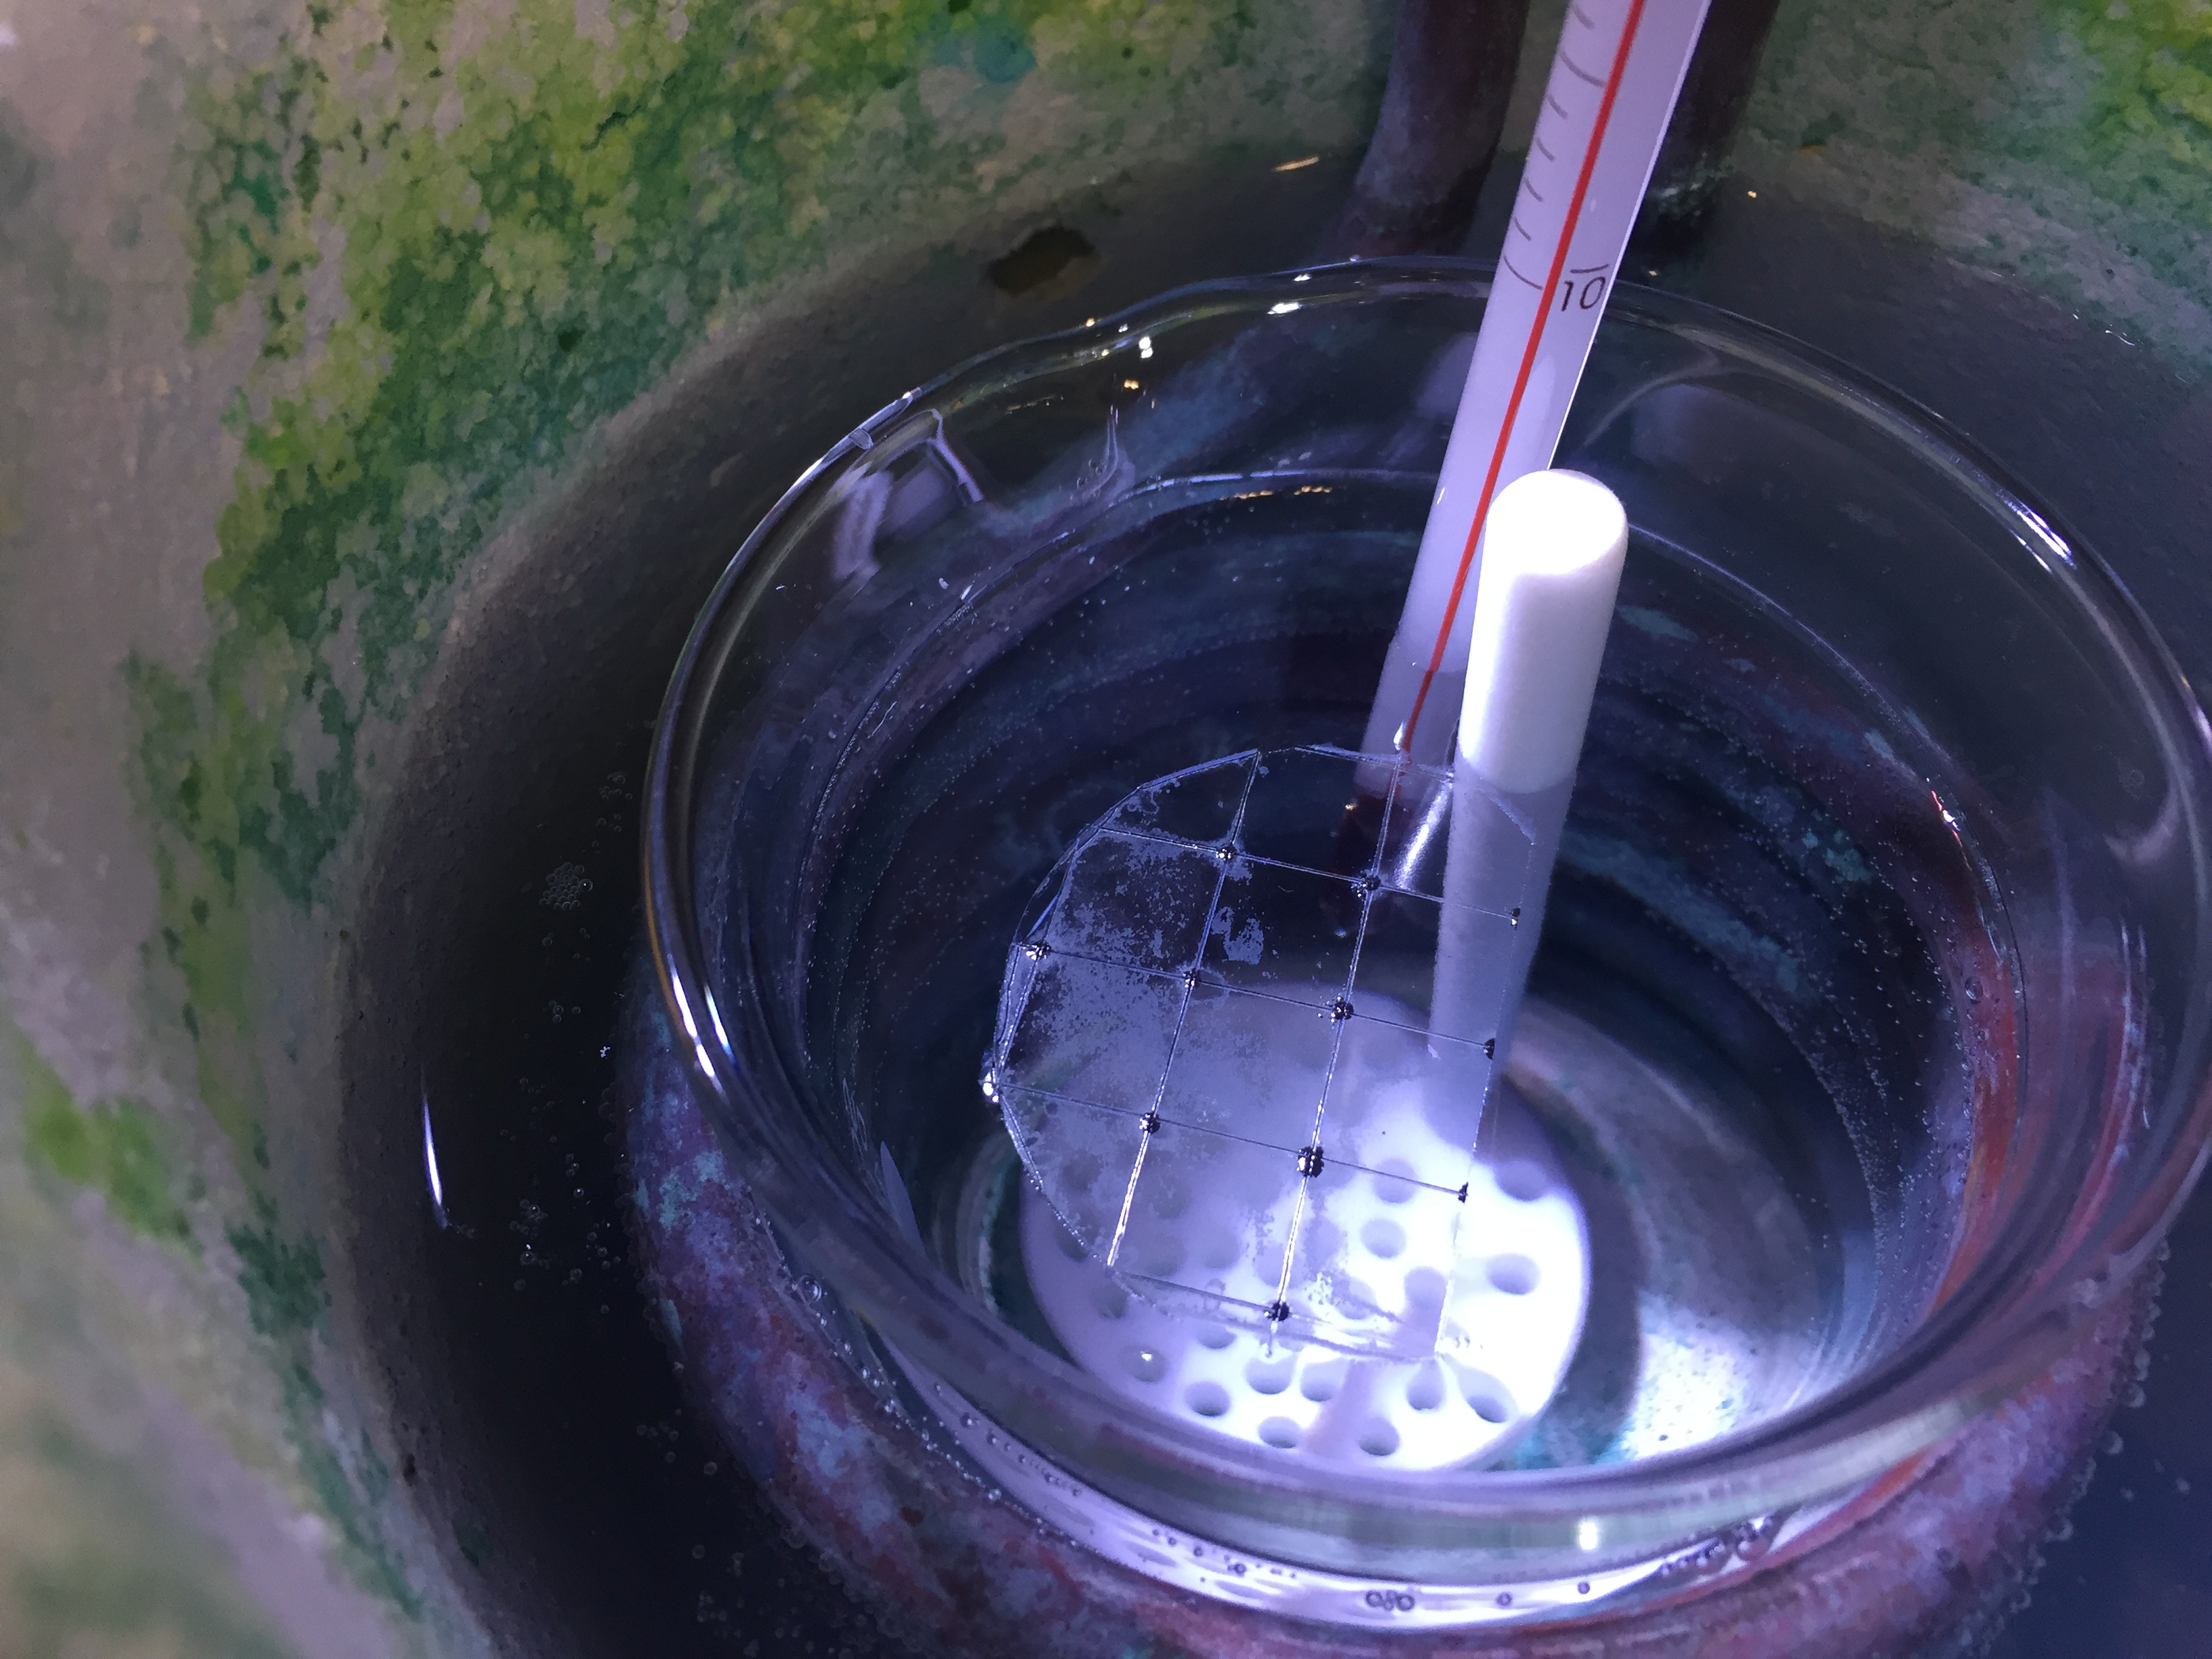
\includegraphics[width=0.45\textwidth]{images/milky_aspects.JPG}
            \label{fig:milky-aspects}}
            \hfill
            \subfloat[]{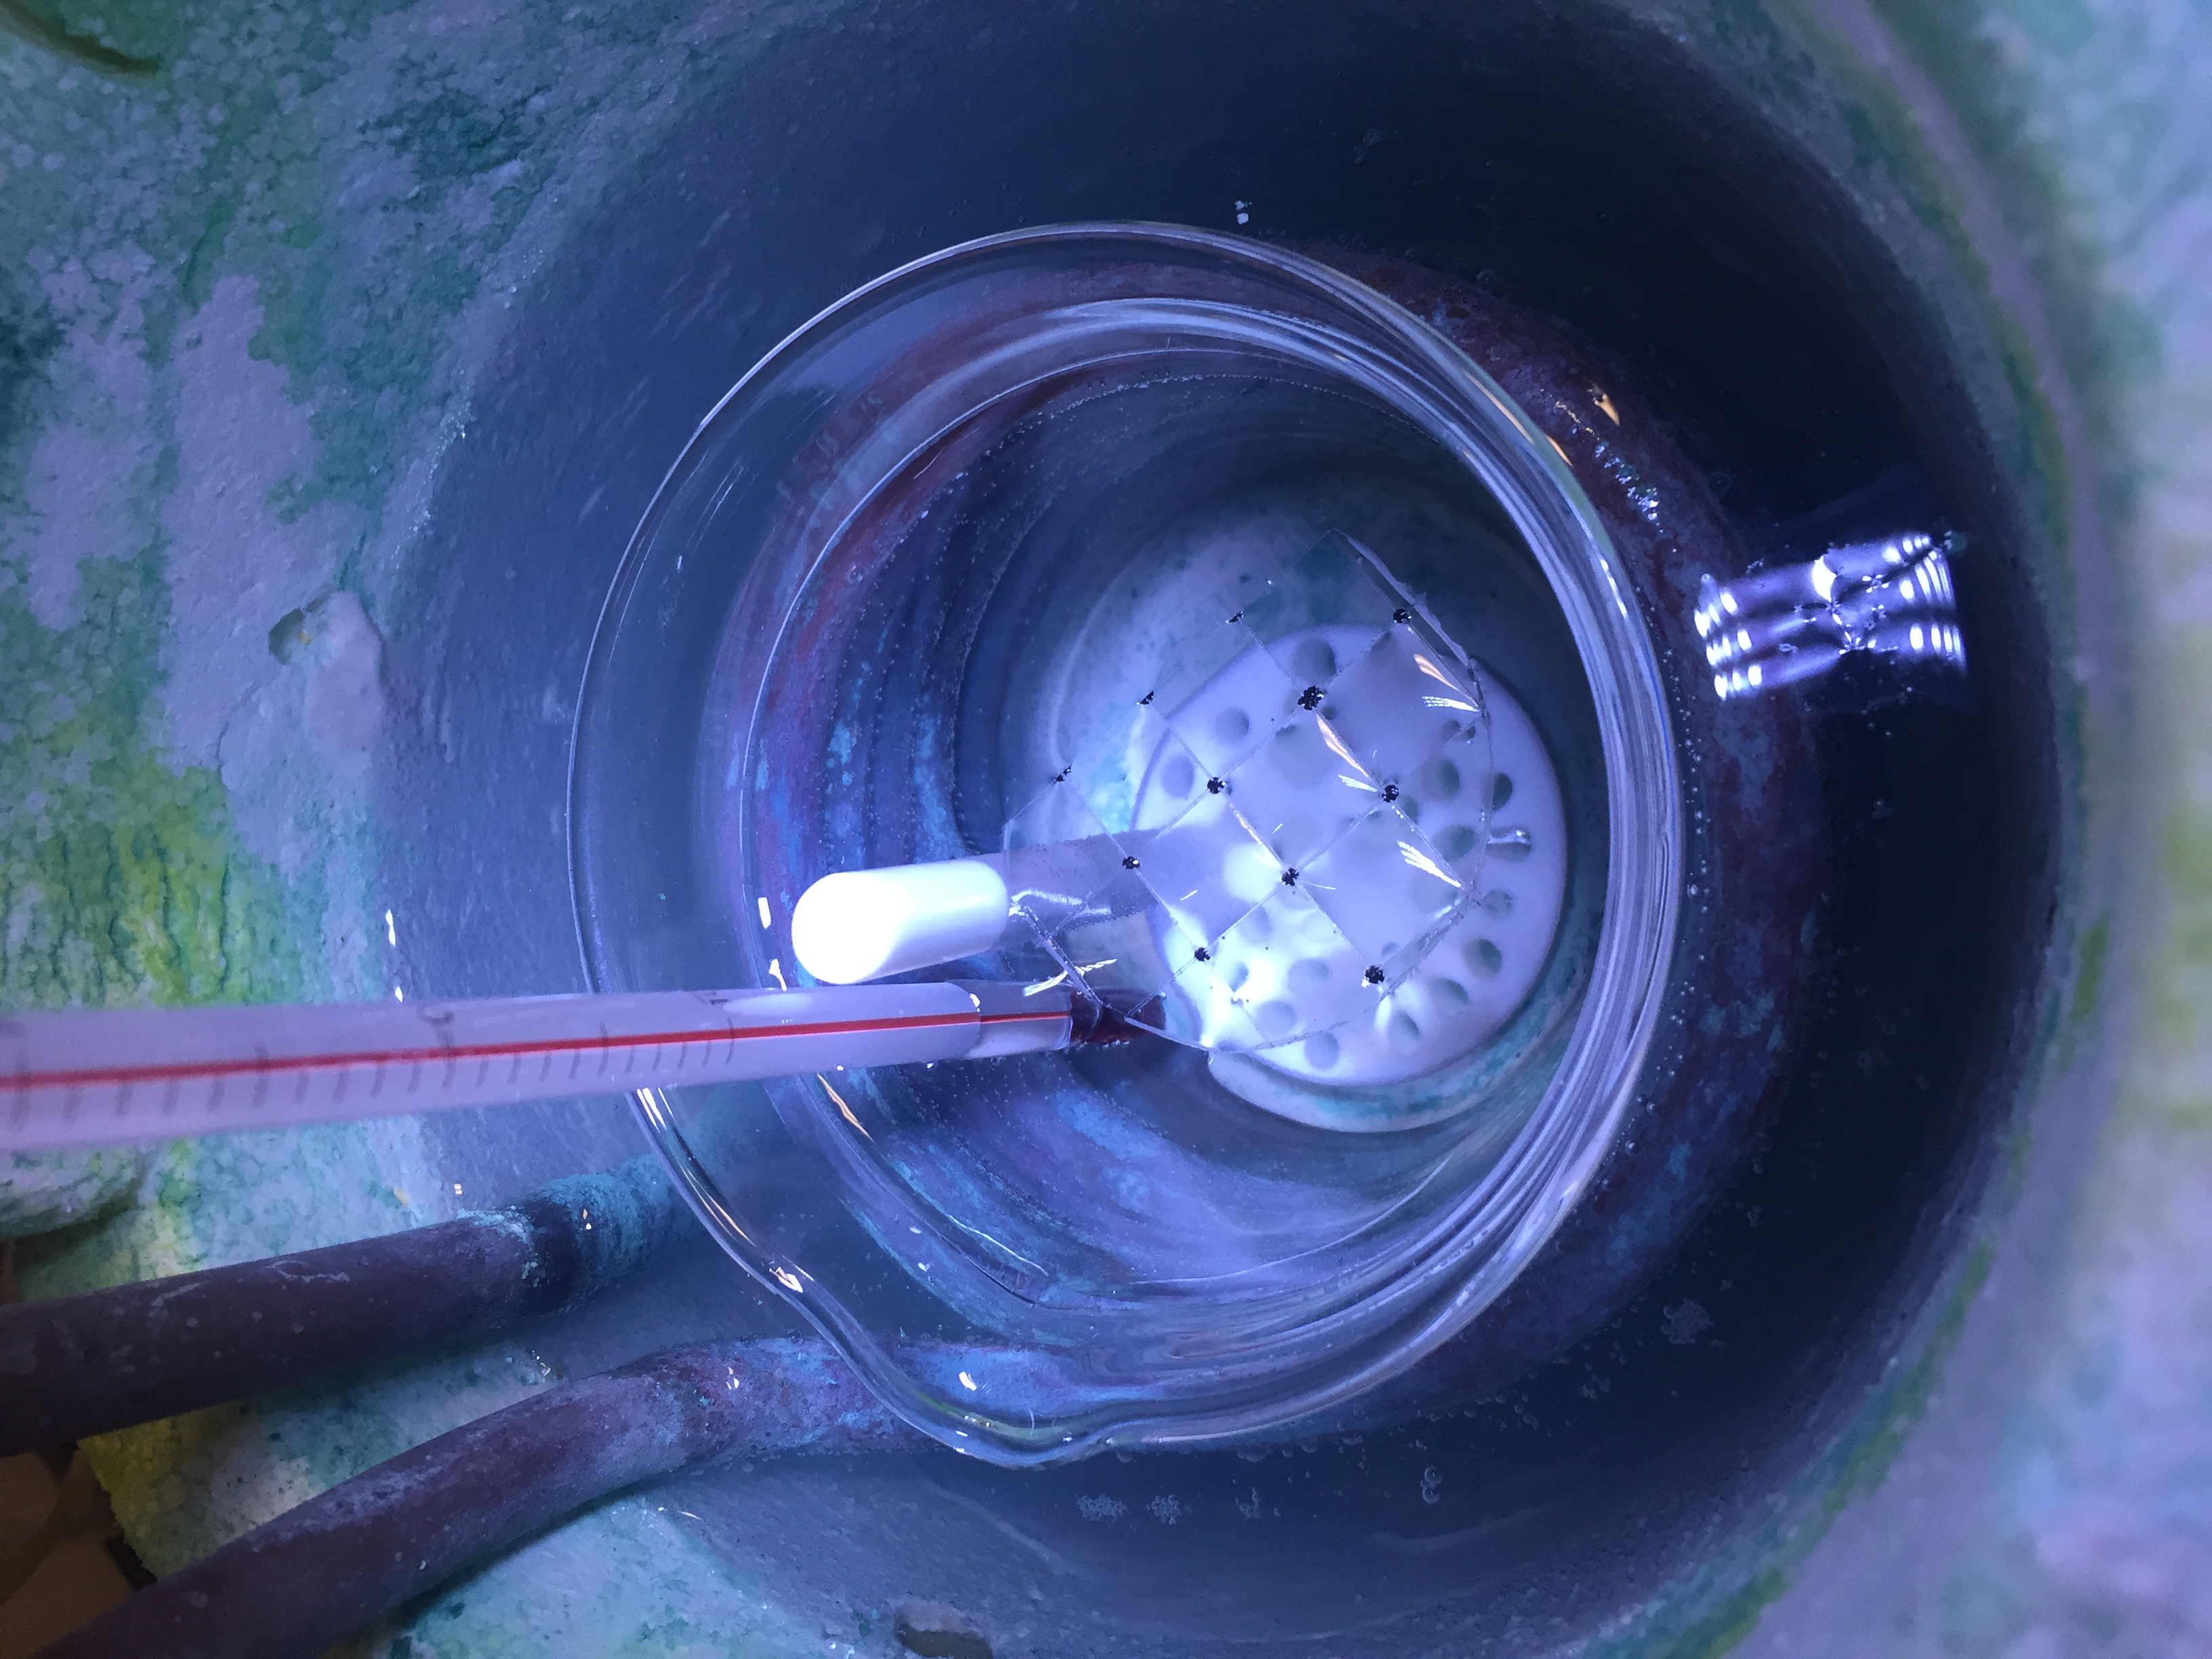
\includegraphics[width=0.45\textwidth]{images/filmed_membrane.JPG}
            \label{fig:filmed-membrane}}
            \caption{Images taken of wafer 295 during the \textit{barrier layer} dissolution process. \protect\subref{fig:milky-aspects} shows milky aspects that appear after approximately twenty minutes while \protect\subref{fig:filmed-membrane} has been taken just before removing the wafer from the acid. At this point the whole surface of the wafer is covered by phosphoric acid that passed through the pores.}
            \label{fig:barrier-layer-diss-images}
          \end{figure}


            \subsubsection{Funnellization of closed pores increased by immersion in phosphoric acid}
            \label{subsec:immersion-experiment}

              Derive and explain etch rate gradient and influence on the pores' shape.
              \medskip

              Understanding the inverse funnelling becomes one of the main goals of the experimens with wafer 296 as it might be used to correct the shapes of the pores of a given membrane. Therefore, immersion experiments where two closed pore membranes are immersed in phosphoric acid for
              \begin{equation}
                \begin{split}
                  t^\mathrm{296c'}_\mathrm{im}=\SI{6,5}{\minute},    \\
                  t^\mathrm{296d'}_\mathrm{im}=\SI{13}{\minute},
                \end{split}
                \label{eq:immersion-times}
              \end{equation}
              and then the shapes of the volumetric isotherms compared to each other and addition with an untreated closed pore membrane. Focus lies on the shape of the isotherms. Small shifts in diameters are of no interest as the inhomogeneity of the pore size distributions of a wafer has been proven already in \cref{sec:wafer-inhomogeneities}.

              \subfile{tikz/graphs/immersion_experiment/immersion.tex}

              \Cref{fig:immersed-comp-w296} compares the volumetric and also the transmission measurements of the immersed membranes 296c and 296d, again adding the untreated membrane 296a. As explained in \cref{sssec:cfp-leo}, condensation and evaporation in a closed funnelled pore occur at equilibrium pressure. Pores that are open on the large end start filling from the bottom and evaporating from the top so, regarding the isotherms in \cref{fig:immersed-comp-w296}, the lower end of the isotherm rising represents the small bottom end of the pores. This lower end of all three isotherms seems to be superimposed while the top end, representing the large open end of the pores, moves to larger diameters for longer immersion times. As the effect seems to occur linearly over the whole length of the pores, the acid seems to be saturating within the pores losing etching power. By \cref{sssec:cfp-leo}, the process can be visually interpreted as a pore straightening as shown in \cref{fig:funneling_increase}. Moreover, the increase of the funnelling aspect seems to be linear at least within the first 13 minutes of the immersion as doubling the immersion time yields double the diameter shift on the volumetric isotherm (compare \cref{eq:t-immerse}). For instance, \cref{tbl:etch_rate} shows the diameter increase of the pores due to the immersion of the membranes in phosphoric acid. Using this data along with the assumption of a linear etch rate gradient along the length of the pore, the respective etch rate can be plotted as shown in \cref{fig:etch_rate_plot}. Here, the parameter $h$ is used as the height within a vertical pore, where $h=\SI{60}{\micro\meter}$ refers to the open top end of a $\SI{60}{\micro\meter}$ long pore that is closed on the bottom side. The effect, that reduces the funnelling aspect of the pores when floating the membranes on phosphoric acid as to dissolve the \textit{barrier layer} shall be referred to as \textit{inverse funnelling} from now on.

              \begin{table}
                \caption{Diameter reduction per minute of immersion derived from the isotherms of the membranes 296a, 296c, 296d.}
                \label{tbl:etch_rate}
                \selectfontsize{10pt}
                \begin{tabu} {X[r]X[r]X[r]}
                  \unitoprule \\
                  \textbf{$t_\mathrm{im} [\si{\minute}]$} & \textbf{$\Delta d_{h=\SI{60}{\micro\meter}} [\si{\nano\meter}]$} & \textbf{$\Delta d_{h=\SI{0}{\micro\meter}} [\si{\nano\meter}]$} \\
                  \unimidrule \\
                  0 &0  &0 \\
                  6,5 &3  &0  \\
                  13  &6  &0  \\
                  \unitoprule \\
                \end{tabu}
              \end{table}

              As for the transmission measurements, the shifts of the beginning of the condensation dip and also the end of the evaporation dips correspond to the interpretation explained above. Ob the other hand, the magnitude difference of the three isotherms' dips cannot be explained, neither interpreted at this point.

              \subfile{tikz/wafer_analysis/funnelling_increase.tex}


            \subsubsection{Inverse funnelling upon barrier layer dissolution}
            \label{subsec:pore-opening-effect}

              Explain that the pores appear to be straightened bc of floating. Refer to the theory, that there are two sorts of alumina (pure and acid  polluted).
              \medskip

              With the conclusions reached in \cref{subsec:immersion-experiment}, it is clear now that indeed, the \textit{barrier layer} dissolution process reduces the funnellization of the pores. One more thing still does not fit into the great picture, though, which is that the kink of the volumetric isotherm of membrane 295b (compare \cref{fig:295b_op_cp_comp}) disappears uppon pore opening. So far, the etch rate has been proven to show a gradient along the length of the pore, but a linear one which cannot account for this type of change in shape.

              Therefore, a different explanation must exist to account for this change. cite the nice book here and explain the two sorts of alumina which are etched at different rates. Check if that can be true ith the thickness of that thing


        \subsection{Etch rate difference}
        \label{subsec:etch-rate-difference}


          \subsubsection{Pore opening widening pores much less than expected}
          \label{subsec:pore-opening-pore-widening}

            The thickness of the \textit{barrier layer} of wafer 292 has been determined to be
            \begin{equation}
              d_\mathrm{barrier-layer}=\SI{30}{\nano\meter}
            \end{equation}
            by elecetron beam microscopy. After having been floated for
            \begin{equation}
              t_\mathrm{float}^\mathrm{292}=\SI{20}{\minute},
            \end{equation}
            milky aspects as shown in \cref{fiFloating experimentg:milky-aspects} appeared. As the latter are assumed to imply that the \textit{barrier layer} is etched off the wafer, this makes for an etch rate of
            \begin{equation}
              e=\SI{1,5}{\nano\meter\per\minute}.
              \label{eq:etch-rate-barrier-layer}
            \end{equation}
            This result is drastically different from the etch rate computed in \cref{subsec:immersion-experiment} and thus raises questions regarding the etch rate of phosphoric acid on alumina.

            Using the result \cref{eq:etch-rate-barrier-layer} for further calculations yields a theroretical pore diameter increse of
            \begin{equation}
              \Delta d_\mathrm{pore}=\SI{22,5}{\nano\meter}
            \end{equation}
            during the fifteen minutes etching of filled pores when disregarding the acid saturation within the pores. Nevertheless, even regarding the saturation, the bottom end of the pores that is exposed to the bulk acid reservoir should be widened dramatically which is not observed on either electron beam microscopy images nor the volumetric measurements. Further analysis on the difference of the etch rate parallel to the pore axis $e_\mathrm{\parallel}$ and perpendicular to the axis $e_\mathrm{perp}$ follows in \cref{subsec:etch-rate-difference}.

            As a way to not increase the distribution of pore diameters on a given wafer, the idea of floating the wafer on acid for a time just short enough to not open any pores, followed by its full immersion in acid has been developed. As to not increase the pores diameter by too much regardless of the acids saturation, the immediate immersion of the whole wafer wihtout prefloating discarded. Again, the acid's etch rate on the \textit{barrier layer} is a prerequisite and shall be deduced in \cref{subsec:etch-rate-difference}.


            \subsubsection{Etch rate of phosphoric acid on alumina not clear}
            \label{subsec:floating-experiment}

              Explan that the shapes of the isotherms are correct, but that no real conlusion could be made due to the bad MEB views.

              \subfile{tikz/graphs/296_a_e_f/296_a_e_f.tex}

              In order to calibrate the etch rate on the \textit{barrier layer} of a give wafer and to try to reduce its thickness in order to immerse the wafer after for the final pore opening, two membranes are floated on phosphoric acid for
              \begin{equation}
                  \begin{split}
                      t^\mathrm{296e}_\mathrm{fl}=\SI{13}{\minute}, \\
                      t^\mathrm{296f}_\mathrm{fl}=\SI{26}{\minute}.
                  \end{split}
                  \label{eq:floating-times}
              \end{equation}
              After, measurements are conducted and the results compared to membrane 296a, which is an untreated membrane in closed pore state, for a reference (\cref{fig:w296-floating-experiment}). While a slight shift in diameter between the floated membranes and the untreated one is visible, this is assumed not to be due to the treatments but rather due to the inhomogeneity of a given wafer. Moreover, the shapes of the isotherm do not show any significant slopewise deviation. Still, as explained before, the membranes could include pores badly open on the \textit{barrier layer} side. Anyways, to probe the thickness of the \textit{barrier layer}, electron beam microscopy is used and along with the cross section, the two sides of the membranes are imaged. Due to the drift that could not be resolve, the attempt to measure the thickness of the \textit{barrier layer} did not work out well as can be seen on \cref{fig:296e-barrier-layer}. On the other hand, the views of the aluminum side of 295e' (\cref{fig:296e-al-side}) confirm that the pores of the membrane remain closed on the bottom side.

              \begin{figure}[htb]
                \centering
                \subfloat[]{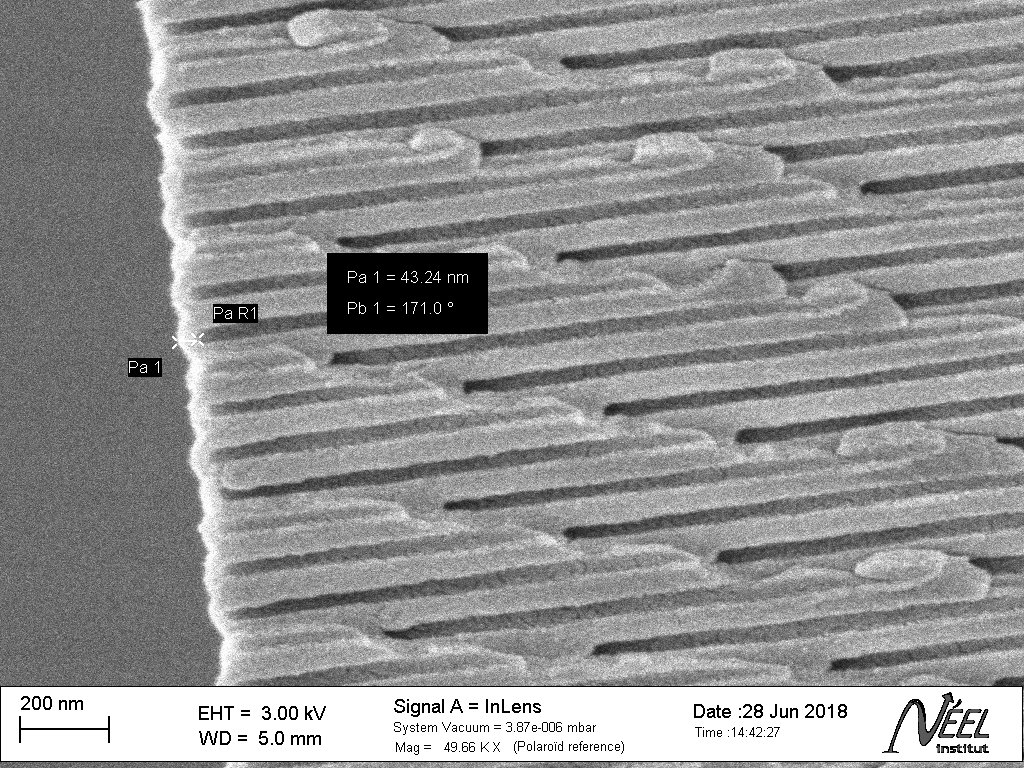
\includegraphics[width=0.45\textwidth]{images/296e_barrier_layer.jpg}
                \label{fig:296e-barrier-layer}}
                \hfill
                \subfloat[]{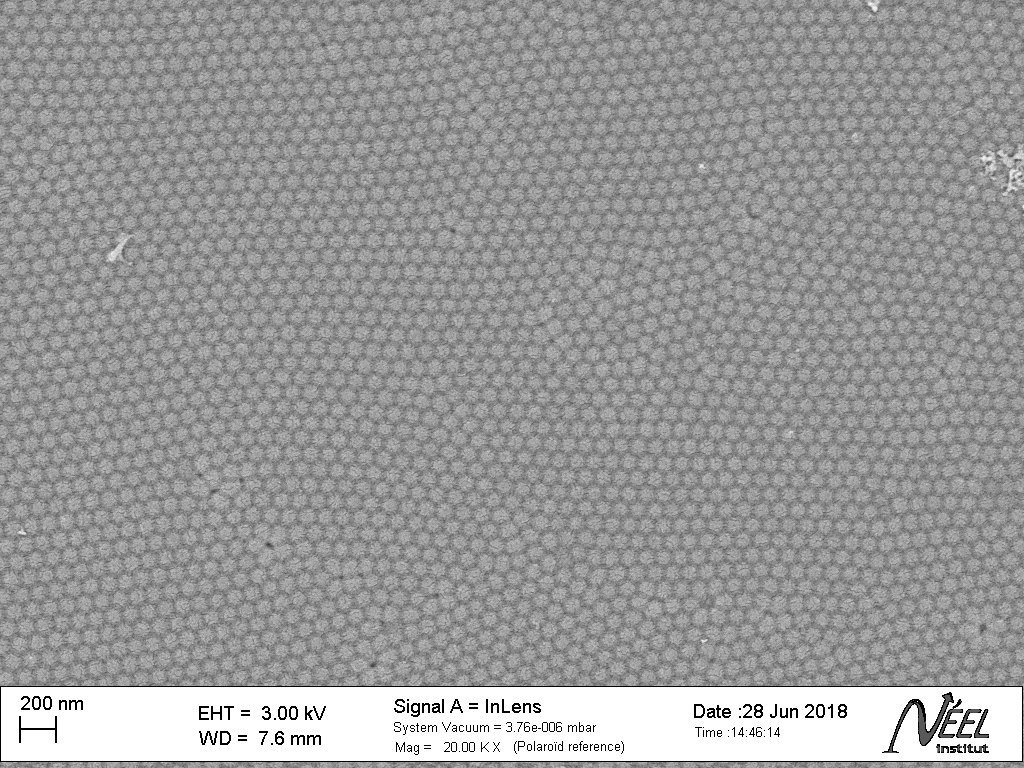
\includegraphics[width=0.45\textwidth]{images/296e_al_side.jpg}
                \label{fig:296e-al-side}}
                \caption{Electron beam microscopy images of membrane 296e' that has been floated on acid for $t_\mathrm{fl}=\SI{13}{\minute}$. \protect\subref{fig:296e-barrier-layer} shows the cross section view with the attempt to measure the thickness of the membrane's \textit{barrier layer}, while \protect\subref{fig:296e-al-side} is the aluminum side on which the membrane has been floated on.}
                \label{fig:floatin-experiment}
              \end{figure}


        \subsection{Do thinner membranes improve things?}
        \label{subsec:thinner-membranes}

          Compare 295 and 296. Talk about the sharpness of both, the volumetric and the optical isotherm. Also speak about the rather broad isotherm for closed pores of 295 which is not understood. Use diameter translation by Kelvin law!!
          \medskip

          Wafer 295 is only
          \begin{equation}
              l^{295}_\mathrm{pore}=\SI{30}{\micro\meter}
          \end{equation}
          thick. Hereby, the effect of the funnelling observed upon the previously measured membranes of a thickness of
          \begin{equation}
              l^{292,293,294,296}_\mathrm{pore}=\SI{60}{\micro\meter}
          \end{equation}
          is expected to be reduced. Assuming that the funneling aspect is linear implies a reduction of the effect by half which should lead to a sharper evaporation branch.

          \subfile{tikz/graphs/295_296_funnelling/295_296_funnelling.tex}

          \Cref{fig:295-296-funnelling-cp} shows the comparison of the membranes 295a and 296b on a \textsc{Kelvin} diameter axis. Both membranes' pores are closed by the \textit{barrier layer} on the bottom side. In contrast to expectations, the evaporation branches show a similar spread
          \begin{align}
            \begin{split}
              \Delta d_\mathrm{evap}^\mathrm{295a}=\SI{15}{\nano\meter} \\
              \Delta d_\mathrm{evap}^\mathrm{296b}=\SI{17}{\nano\meter}.
            \end{split}
          \end{align}
          To determine the latter, the volumetric isotherms' rise and also the transmission drops have been regarded. At this point, assuming some uncertainty also due to the slightly different values derivable from optics and volumetrics, the funnelling aspect seems unchanged by moving to thinner membranes. But, looking at the condensation branches of the volumetric isotherms could bring clarity. While the condensation branch of membrane 296b shows approximately the same slope and shape as its evaporation branch, for membrane 295a this is not true. The latter membrane's condensation branch spreads out over about $\SI{25}{\nano\meter}$ so it is much broader than its evaporation branch. This can only be explained by severe corrugations within the pores as straight funnelling should not cause any differences in shape between the condensation and evaporation branches according to \cref{sec:cond_evap_theory}. The transmission signals match in magnitude for both membranes while it is much sharper for the thinner one. As a first guess, this could be interpreted as a sign more less flawed or even less corrugated pores, though that would contradict the before made analysis. In conclusion, from the closed pore isotherms no conclusion can be drawn as to how the funnelling aspect is affected by reducing the membrane thickness.

          \Cref{fig:295-296-funnelling-op} then shows the isotherm comparison of the open pore membranes 295g' and 296b'. For these isotherms, the condensation does match the evaporation branch shapewise. The spread of the evaporation is
          \begin{align}
            \begin{split}
              \Delta d_\mathrm{evap}^\mathrm{295g'}=\SI{9}{\nano\meter} \\
              \Delta d_\mathrm{evap}^\mathrm{296b'}=\SI{13}{\nano\meter}.
            \end{split}
          \end{align}
          Again, the transmission drops for the thirty micrometer membrane 295g' are more sharp but within the same magnitude as those of 296b'. A difference in funnelling seems more probable from this measurement even though, the bottom line is that no precise conclusion can be drawn from the measurements at this point.

          For more calrity, electron beam microscopy is used to check the difference of the diameters on solution and aluminum side. \Cref{fig:meb-funnelling} shows the images for the membranes 295g' and 296b' which state a diameter offset of about
          \begin{align}
            \begin{split}
              \Delta d_\mathrm{sem}^\mathrm{295g'}=\SI{6}{\nano\meter}, \\
              \Delta d_\mathrm{sem}^\mathrm{295g'}=\SI{6}{\nano\meter}.
            \end{split}
          \end{align}
          So the SEM images show the same tendency as the volumetric and optical measurements.
          \medskip

          \begin{figure}[htb]
            \centering
            \subfloat[]{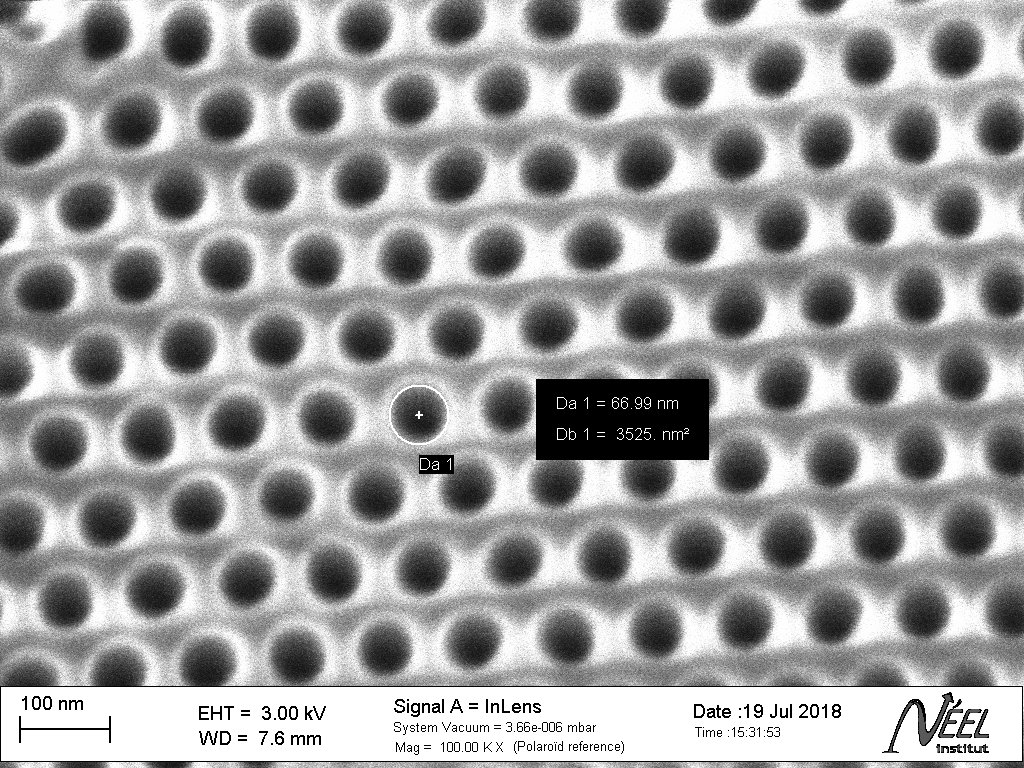
\includegraphics[width=0.45\textwidth]{images/296g_sol_side.jpg}
            \label{fig:295g-sol-side}}
            \hfill
            \subfloat[]{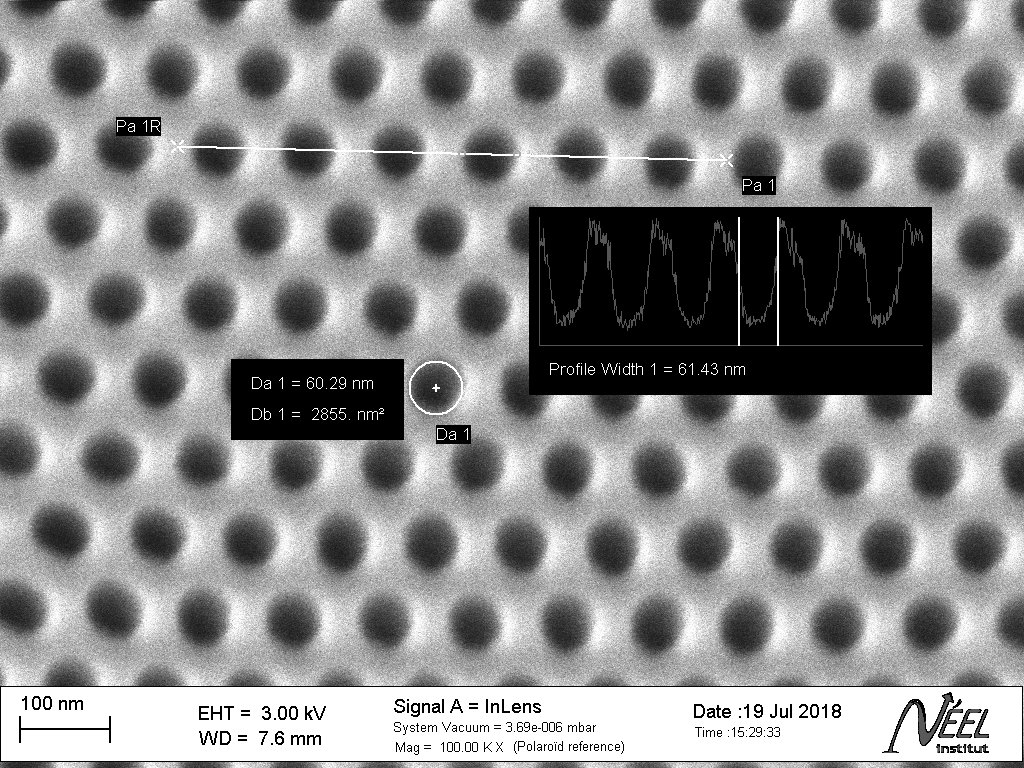
\includegraphics[width=0.45\textwidth]{images/296g_al_side.jpg}
            \label{fig:295g-al-side}}
            \caption{Electron beam microscopy images of membrane 295g' with measurements of the pore diameters on the solution side \protect\subref{fig:295g-sol-side} and aluminum side \protect\subref{fig:295g-al-side}.}
            \label{fig:meb-funnelling}
          \end{figure}

          To conclude with, even though the effect is not as significant as expected, thinner membranes indeed do improve the pore quality.


        \subsection{Transmission signal not well understood}
        \label{subsec:transmission-mysteria}

          To begin with it must be mentioned here, that all open pore membranes measured before the wafers 295 and 296 have shown the same transmission characteristics in regard of the significant magnitude difference of the condensation and evaporation isotherm branch which can be seen on \cref{subfig:292-trans}. Therefore, a theory to explain this phenomenom were developed. The prominent one at the beginning of the conducted experiments mentioned in this report shall be explained in the following.

          \subfile{tikz/graphs/292_295_296_transmission/292_295_296_transmission.tex}

          Firstly, a completely filled membrane should always yield a higher transmission coefficient $T$ than it would in its dry state according to the theory of index matching explained in \cref{sec:index-matching}. This fact serves as a tool to optically detect membranes that do not fill completely due to constrictions which by experience show a weaker tranmission after the condensation process is complete than they did before. Furthermore, due to the disorder created by pore filling and emptying, the transmission drops during the processes. Phenomena occurring on the volumetric measurements can therefore be linked to the measured transmission coefficient.

          Moreover, the phenomenom of the transmission dropping to lower values for the condensation than for evaporation branch of a given isotherm has been repeatedly observed on open pore membranes. An example is given by membrane 292d's isotherm whcih is displayed in \cref{fig:292-trans}. At this point it must be mentioned that all open pore membranes measured before the wafers 295 and 296 have shown this same transmission characteristics. As interpretation serves the degree of disorder caused inside the membrane by the respective process. As the membrane contains pores open on both ends, the condensation occurs at spinodal pressure $P_\mathrm{sp}(d_\mathrm{pore})$. Due to the distribution of pore sizes, funnelization, corrugation and constrictions, the pores fill at different pressures $P_\mathrm{sp}^1 \neq P_\mathrm{sp}^2$. At a given pressure
          \begin{equation*}
              P_\mathrm{sp}^1 < P < P_\mathrm{sp}^2,
          \end{equation*}
          where $P_\mathrm{sp}^1$ shall correspond to the smallest pore diameter found on the membrane and $P_\mathrm{sp}^2$ the largest one, the state of the me{}mbrane regarding filled and empty pores is assumed to be comparable to figure \cref{fig:disorder-absorption}. The hexane evaporates at equilibrium pressure $P_\mathrm{eq}$, though. That means that, assuming the same pore size distribution, funnelization, corregation and constrictions, the pores empty continuously. The theoretical state of the membrane is visualized in \cref{fig:disorder-desorption}.

          The difference is given by the most significant contrasts between neighboring pores during the condensation process, in explanation empty and filled pores, for spinodal condensation, while for evaporation at equilibrium pressure the pores only show different levels of liquid during most of the process. As a result, the absorption of hexane creates a higher grade of disorder than the desorption and therefore causes a more significant drop of the transmission coefficient (compare \cref{fig:292-trans}).
          \medskip

          The splitting of the evaporation drop into two dips seperated by a small local maximum cannot be explained by this theory, nor by any other means mentioned in this report. Moreover, the later analysed membranes of wafer 295 and 296 yield a more even dip distribution (compare \cref{fig:295-trans} and \cref{fig:296-trans}) and upon reducing the pore diameter of 295 using ALD, the membranes even show the inverse behaviour (\cref{fig:295f200ALD-trans}).

          In connection with the sharper isotherms, the first phenomenom could be explained by the pores being less flawed talking corrugations and funneling. The latter assumption is backed by the fact, that the transmission drops of 295d are of smaller magnitude than those of 296b. While both are open pore membranes, membrane 295d is only half as thick as 296b, meaning the pores are only half as long and therefore the influence of the funneling aspect is reduced as will be explained in \cref{subsec:thinner-membranes}.

          The second phenomenom of the deeper evaporation dip remains unclear though.

          \subfile{tikz/transmission_disorder/pore_disorder.tex}


      \section{Pore quality linked to transmission drop and hysteresis}
      \label{sec:pore-quality-link}

        As of now the shapes of the isotherms are more familiar to the reader, at this point the isotherms of the open pore membranes of wafer 295 are analysed in more detail. For this please refer to the isotherms shown in \cref{fig:295-op} of \cref{sec:wafer-inhomogeneities}. There are two isotherms that sting the eye as they do not blend in: The membranes 295c' and 295d'. Again, the analysis of membrane 295c' shall be postponed. Focusing on 295d' shows that its isotherm is not only shifted to larger pressures in comparison to the other membranes, but also is the hysteresis smaller. Moreover, the transmission drops are of a smaller magnitude for membrane 295d' than for all others. As the pressures translate to diameters
        \begin{equation}
          d_\mathrm{pore}> \SI{60}{\nano\meter},
        \end{equation}
        \textsc{Kelvin} equation is assumed to be sufficiently correct. The isotherms of the membranes 295d' and 295g', which is from here on used as a representative of the rest of the open pores membranes of wafer 295, are plotted over a diameter axis in \cref{fig:295-d-g}. Interesting at this point is, that hysteresis is actually smaller for membrane 295g' on a \textsc{Kelvin} diameter scale. Also, the evaporation branch seems sharper which could account for less funnelled pores.
        \medskip

        Very weird stuff here... HELP???

        \subfile{tikz/graphs/295_d_g/295_d_g.tex}


      \section{Testing theory using electron beam microscopy}
      \label{sec:testing-theory}


      \section{Pore size reduction using atomic layer deposition}
      \label{sec:ald-experiments}

        Finally, as the open pore membranes of wafer 295 prove to be very good in the sense of producing very sharp isotherms and showing similar diameters, the goal of sub ten nanometer pore diameters is resumed. The pore diameters are reduced using atomic layer deposition (ALD). \Cref{fig:wafer_295} shows the treatments and measurements of the inspected membranes of wafer 295.

        \subfile{tikz/graphs/295e_ALD/295e_ALD.tex}


        \subsection{Atomic layer deposition effectively reduces pore diameters}
        \label{subsec:ald-reduces-diameters}

          The first important question is if ALD works to serve as a diameter reduction at all. Therefore, on membrane 295e' 100 cycles of ALD are conducted and the membrane then probed using the experimental setup and SEM. The measurement results are shown in \cref{fig:295e-ald}. While the result for the first 100 cycles of ALD matches expectations perfectly, the second 100 cycles give a very different impression, though, and its result's discussion shall be postponed in favor of the analysis of 295e' and 295e'' at this point.

          Firstly, the shape of the volumetric isotherm does not change for membrane 295e'' in comparison to 295e'. It is only shifted towards lower pressures. Only the hysteresis increases by a little bit which can be explained by the logarithmic context of realtive pressure to pore diameters though. Regarding the isotherms of 295e' and 295e'' on a \textsc{Kelvin} diameter axis as shown in \cref{fig:295e-ald-kelvin}, the change of the hysteresis disappears and the evaporation branches show the same steepness for both membranes. Furthermore, the diameter reduction by 100 cycles of ALD according to the isotherms is
          \begin{equation}
            \Delta d_\mathrm{pore}^\mathrm{295e'\rightarrow 295e''}=\SI{20}{\nano\meter}
          \end{equation}
          which makes for
          \begin{equation}
            \Delta =\SI{0,2}{\nano\meter}
          \end{equation}
          diameter reduction per ALD cycle. This value matchs the expectations of
          \begin{equation}
            \Delta = \SI{0,2}{\nano\meter}
          \end{equation}
          per cycle as explained in ???.

          The tranmission measurements also yield very sharp drops for the membranes 295e' and 295''. One phenomon, which has not been observed before, is that the evaporation transmission drop of membrane 295e'' is deeper than its condensation transmission drop. This does not go together with the theory for the before observed inverse phenomenom as explaind in \cref{subsec:transmission-mysteria}. Up to this point, no explanation could be found for the observation.


        \subsection{Diameter reduction by atomic layer deposition is reproducible}
        \label{subsec:diameter-reduction-reproducible}

          Next, membrane 295e''' and 295f'' must be compared to probe the reproducibility of the pore diameter reduction using atomic layer deposition. As on the one hand the membranes 295e' and 295f' yielded equivalent measurement results as can be seen in \cref{fig:295-op} and on the other hand both, 295e''' and 295f'', have undergone 200 cycles of ALD in total, their measurements should produce very similar results.

          The measured data is plotted in \cref{fig:295-e-f-ald}. While the overall picture of the two membranes seems to match, clearly there is a shift towards lower pressures visible for membrane 295f''. Anyways, the membranes used for this comparison both show isotherms that do not match expectations and imply that the atomic layer deposition did not work out properly. As, according to \cref{subsec:ald-reduces-diameters}, it works for only 100 cycles and also the result seems independent of the ALD process being interrupted during the full 200 cycles, leads to the conclusion that something is off for smaller diameters which will be further analysed in the following section. Talking reproducibility, a tendency towards yes is justifiable but needs to be confirmed through further experiments.

          \subfile{tikz/graphs/295_e_f_ALD/295_e_f_ALD.tex}

          \subsection{Atomic layer deposition parameters need improvement}
          \label{parameters-need-improvement}

            \subfile{tikz/graphs/295_e_f_ALD/295e_200ALD.tex}

            In the following, the transition from membrane 295e'' to 295e''' using 100 layers of ALD shall be tried to understood. \Cref{fig:fig:295-e-200ald} shows the measured isotherms over a relative pressure axis. The condensation in two steps together with a one step evaporation hint at a population of closed or constricted pores. Therefore, the isotherms are plotted on a \textsc{Kelvin} diameter axis in \cref{fig:295-e-200ald-kelvin} twice, once using the conversion for open pores (cylindrical meniscus) and once that closed pores (spherical meniscus). A black circle marks where the two steps of the isotherm's condensation branch superimpose on the same diameter range as a result. Moreover, another circle marks the corresponding transmission drops. They are both shifted towards higher pore diameters in comparison to the volumetric signals of condensation, but still, they are aligned on top of each other. These observations back the suspicion of closed or constricted pores.
            \medskip

            \subfile{tikz/graphs/295_e_f_ALD/295f_200ALD.tex}

            \begin{figure}[tpb]
              \centering
              \subfloat[]{
                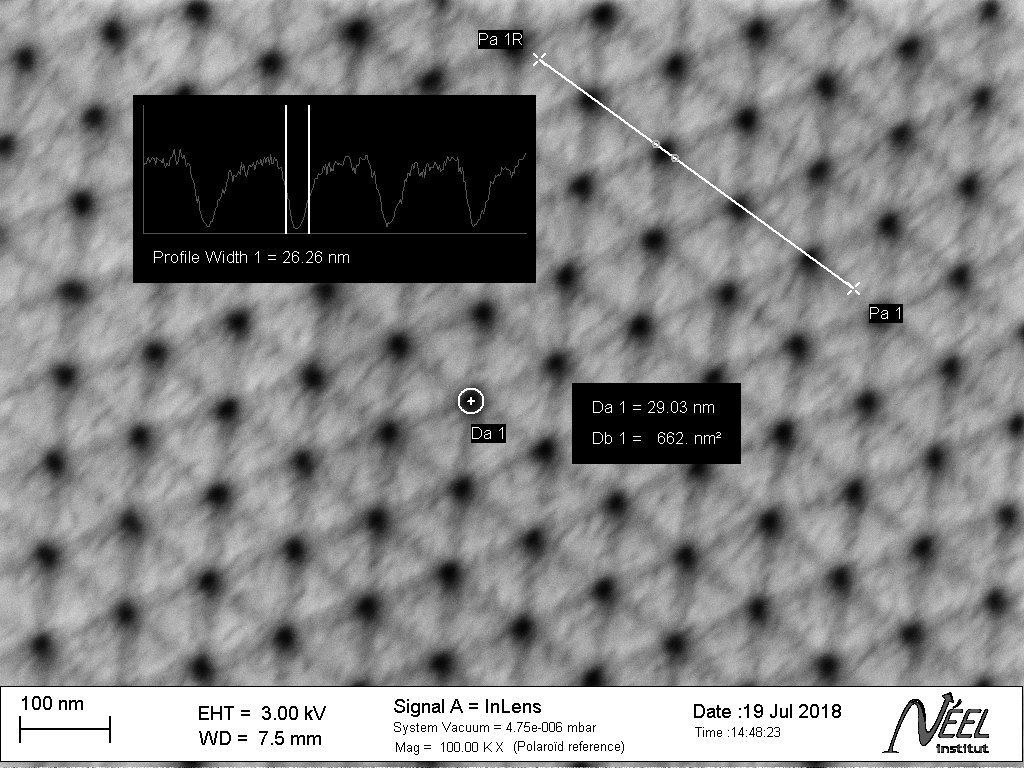
\includegraphics[width=0.45\textwidth]{images/295f_200ALD_sol_side.jpg}
                \label{fig:295f-200ald-sol-side}
              }
              \hfill
              \subfloat[]{
                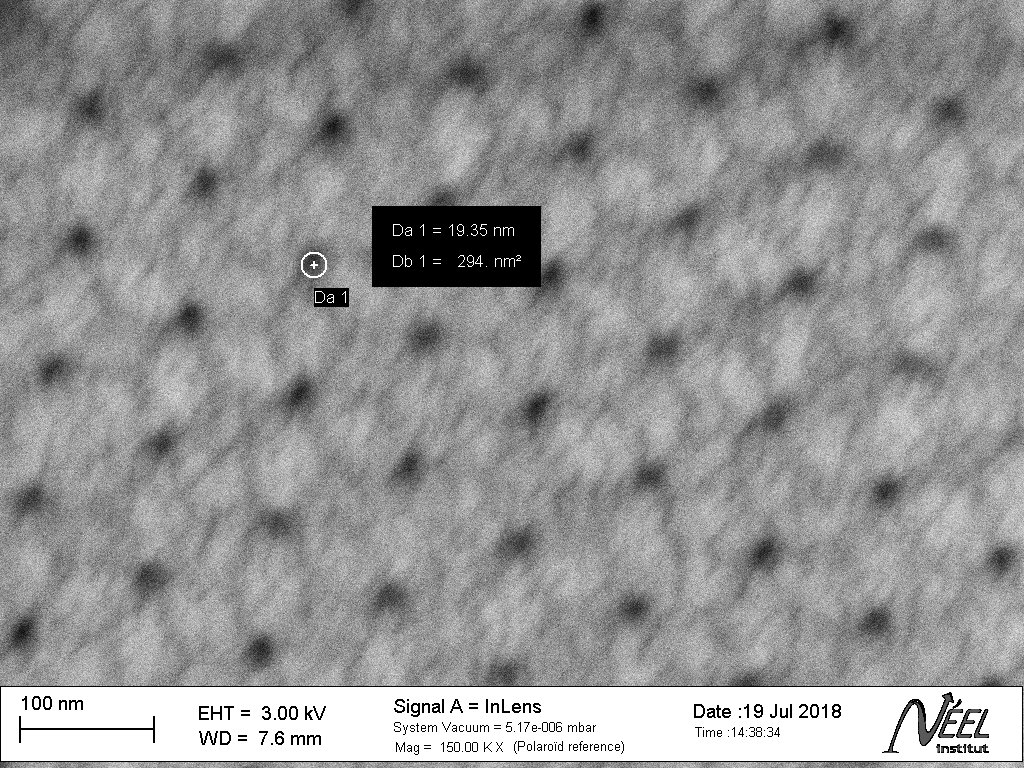
\includegraphics[width=0.45\textwidth]{images/295f_200ALD_al_side.jpg}
                \label{fig:295f-200ald-al-side}
              }
              \\
              \subfloat{
                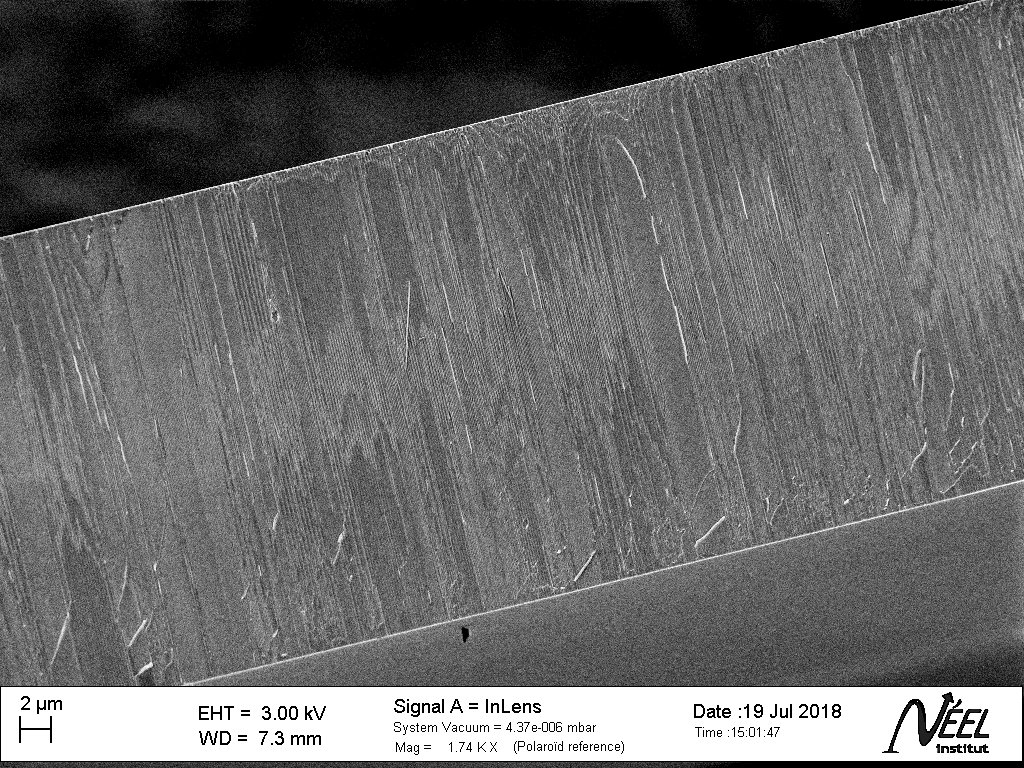
\includegraphics[width=0.9\textwidth]{images/295_gradient.jpg}
                \label{fig:295f-gradient}
              }
              \caption{Electron beam microscopy images of membrane 295f'''. \protect\subref{fig:295f-200ald-sol-side} and \protect\subref{fig:295f-200ald-al-side} show images of the solution and aluminum side with pore diameter measurements. \protect\subref{fig:295f-gradient} captures the grayscale gradient on the membrane's cross section which gets lighter upon approaching the center from both sides.}
              \label{fig:295f-200ALD-sem}
            \end{figure}

            Already in \cref{subsec:diameter-reduction-reproducible}, the similarity between the results of the membranes 295e''' and 295f'' has been analysed. For the sake of completeness, the same analysis as for membrane 295e''' shall be done here. Again, the two step condensation together with the single step evaporation hint at closed or constriced pores. Using \textsc{Kelvin} equation to convert the relative pressure to diameters for closed and open pores yields the same superposition as observed for membrane 295e''', again marked by black circles for volumetrics and optics. In addition to the volumetric and the transmission measurements, for membrane 295f'' SEM images have been taken. \Cref{fig:295f-200ald-sol-side} and \cref{fig:295f-200ald-al-side} show the solution and aluminum side of the membrane. The pore diameters of
            \begin{equation}
              \begin{split}
                  d_\mathrm{pore,SEM}^\mathrm{295d'',Sol}=\SI{27}{\nano\meter}, \\
                  d_\mathrm{pore,SEM}^\mathrm{295d'',Al}=\SI{27}{\nano\meter}
              \end{split}
            \end{equation}
            approximately match the diameters derived from the condensation branches of the volumetric isotherms whereas the evaporation branch would imply pore diameters of about
            \begin{equation}
              d_\mathrm{pore,evap}^\mathrm{295d''}=\SI{10}{\nano\meter}.
            \end{equation}
            Up to this point though, the evaporation branch has been assumed to be more precise for measuring the pore diameters as it only depends on equilibrium pressure.

            ??? KELVIN IS NOT RELYABLE AT THESE LOW DIAMETERS - RATHER TRUST EVAPORATION -> constricted pore ends ! CHECK FOR CONDENSED LIQUID AND COMPARE TO EXPOECTATION!!!
            \medskip

            Finally, \cref{fig:295d-200ALD} shows the isotherm data for membrane 295d''. While there is still a volumetric signal visible, its pressurewise position does not match expectations as the deposit of 250 layers should make for smaller pores than the 200 layer on the membranes 295e''' and 295f''. Therefore, the signal might very well just be due to noise of the measurements. On the other hand, Also the transmission signal shows a drop. The signal does not rise again even at saturated vapor pressure though. The latter observation implies constricted pores that do not fill at all.

            \subfile{tikz/graphs/295d_ALD/295d_250ALD.tex}


      \section{Isotherms proves powerful to detect and characterize defects}
      \label{sec:theory-and-defects}

        \subfile{tikz/graphs/295c/295c.tex}

        Throughout the data evaluation, the volumetric measurements along with the laser transmission prove extremely sensitive to detect pore defect like closed pores, where they should be open, constrictions at the pore ends, corrugations or even funnellization. As a last example, membrane 295c' shall be analysed and the result applied to the other membranes of wafer 295.

        Expectations are that membrane 295c' shows the same properties as the other open pore membranes of wafer 295 as they were all floated on phosphoric acid still attached to the initial wafer except for 295b'. \Cref{fig:295c} displays its isotherm. In contrast to expectations, the isotherm shows a three step condensation branch while the evaporation branch consists of a single drop. An evaporation at high pressures that consists of a single sharp drop implies that all pores are distributed around a single diameter. As a consequence, the isotherm is plotted over pore diameters $d_\mathrm{pore}$ using \textsc{Kelvin} equation (\cref{sec:kelvin-equation}) for closed pores and open pores seperately and superimposed in one coordinate system (\cref{fig:295c-op-cp}). As the black circle tries to focus on, the first small rise at low pressures translates to the same pore diameter as the second one does for open pore analysis. This hints at a small population of closed pores on the wafer. In fact, the MEB images of the aluminum side of membrane 295c shown in \cref{fig:295c-meb} actually do show areas of none open pores which fill at equilibrium pressure which is coherent with the before made assumptions based on the volumetric isotherms. Moreover, regarding the laser transmission signal, another phenomenom implying pores filling at equilibrium pressure an be found. As amplified in \cref{fig:295c}, the transmission drops at about the same pressure as the first liquid fraction rise finishes and stays at this lower value until the occurence of the spinodal condensation where it drops farther. This drop can be explained by some pores filling and scattering light as a result as before explained in \cref{subsec:light-transmission-interpretation} referring to \cref{fig:disorder-absorption}.

        As for the third rise of the volumetric isotherm's condensation branch, it can be explained by pore size distribution of open pores with two peaks. As there is no known reason for this kind of distribution, this explanations seems unlikely though. At this point, no other interpretation has been concluded with.
        \medskip
        Now assuming that



        \begin{figure}[htpb]
          \subfloat[]{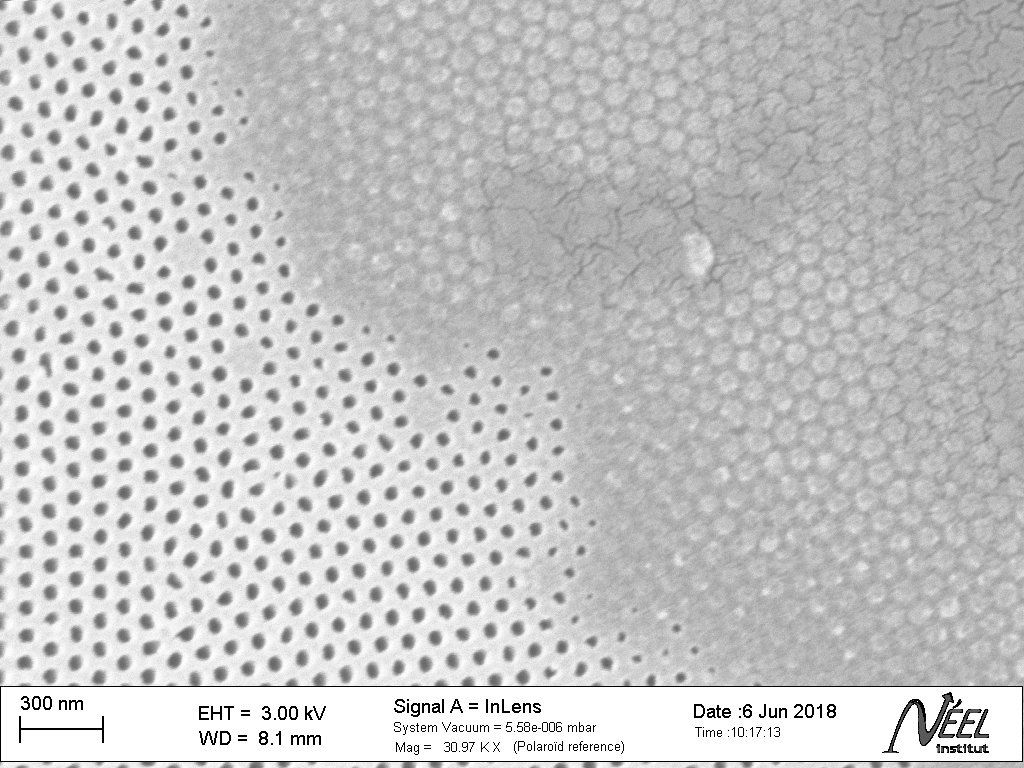
\includegraphics[width=0.45\textwidth]{images/295c_al.jpg}}
          \hfill
          \subfloat[]{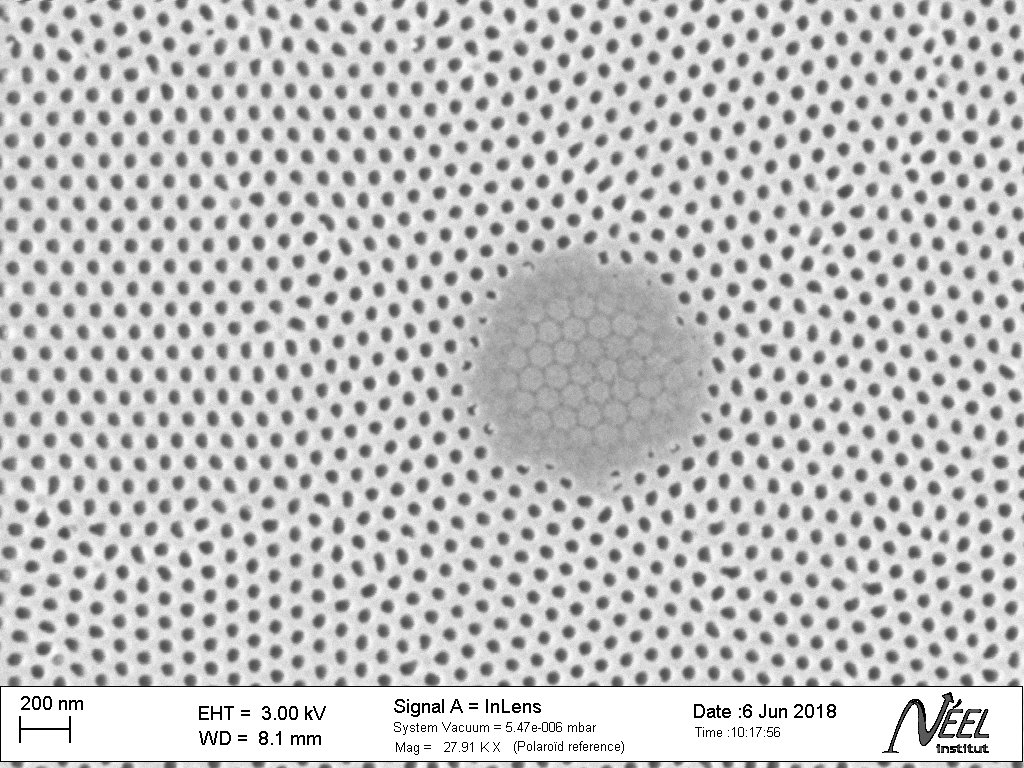
\includegraphics[width=0.45\textwidth]{images/295c_al_2.jpg}}
          \caption{MEB images of the aluminum side of membrane 295c. Areas of none open pores are clearly visible.}
          \label{fig:295c-meb}
        \end{figure}

      \medskip

      Bring up membrane 293 (constricted pore ends) and membrane 295c (closed pores).
      MAYBE PUT THIS IN THE CONCLUSIONS CHAPTER???


\end{document}
